\section{Aufbau}
\begin{frame}{Aufbau}
    \begin{itemize}
        \item Bodenstationen
        \item[]~
        \item Satelliten
    \end{itemize}
\end{frame}

\begin{frame}{Bodenstationen, {\small [gps.gov]}}
    \begin{figure}
        \centering
        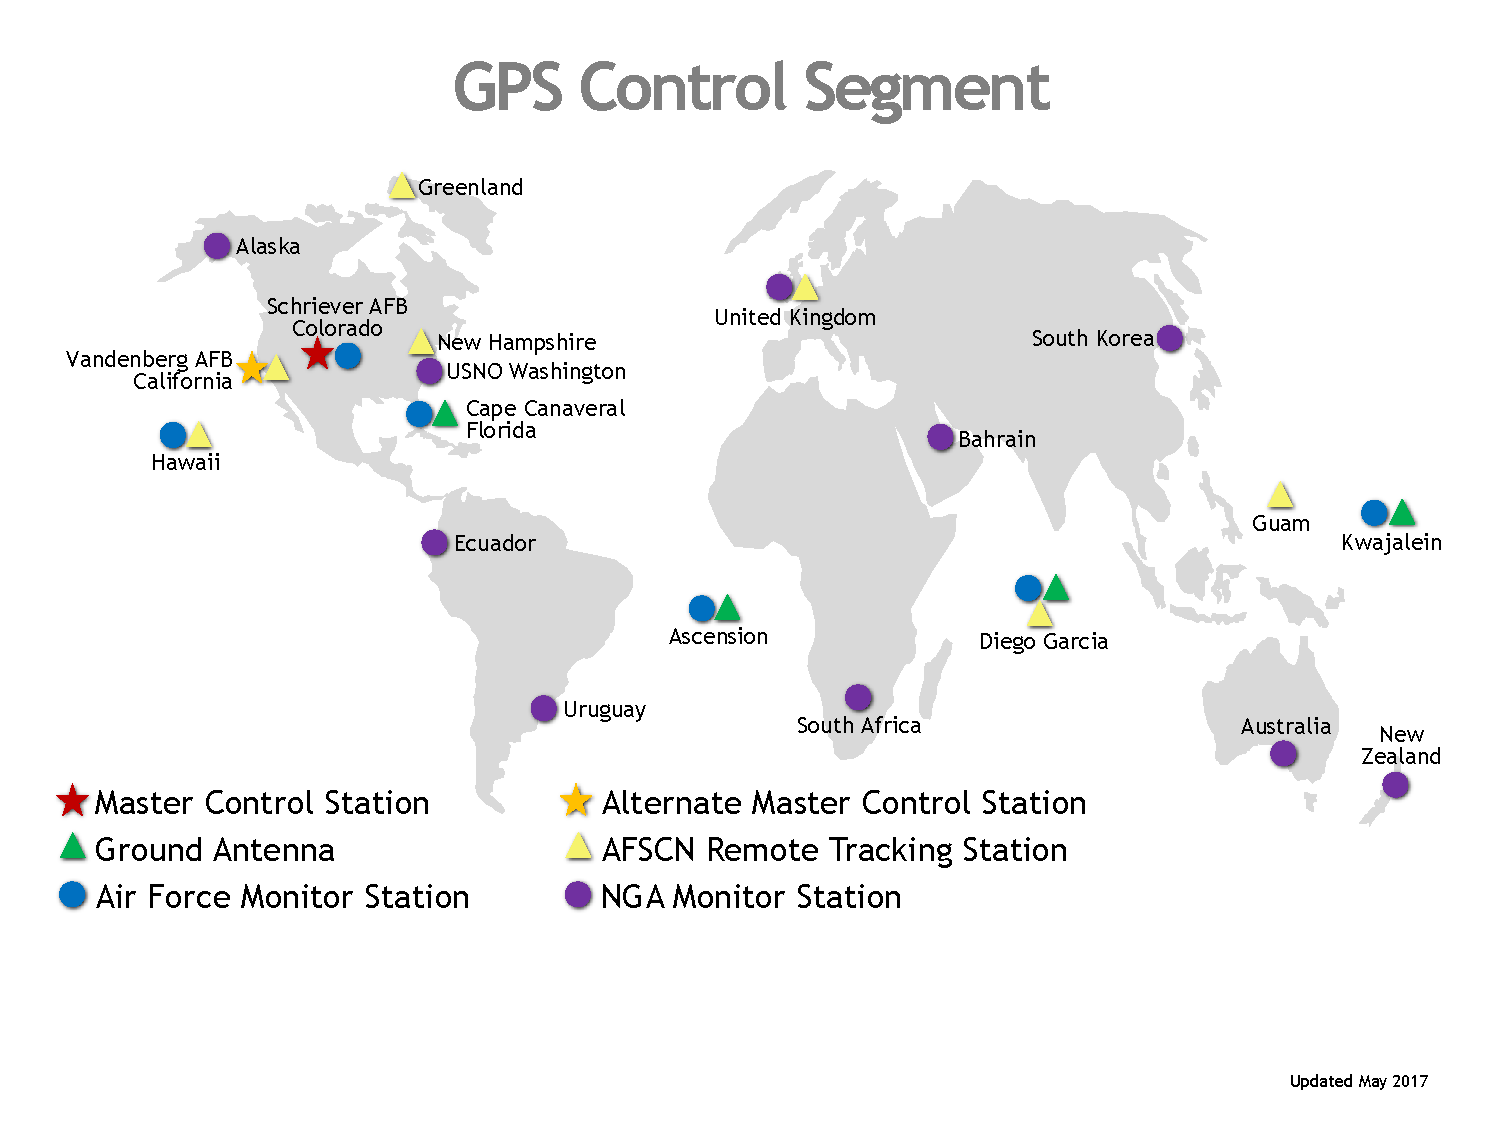
\includegraphics[width=\textwidth]{images/GPS-control-segment-map.pdf}
    \end{figure}
\end{frame}

\begin{frame}{Konstellation}
    \begin{columns}
        \begin{column}{0.5\textwidth}
            \begin{itemize}
                \item[Höhe:] \SI{20200}{\kilo\meter}
                \item[Umläufe:] 2 pro Tag
                \item[Orbitale:] 6, mit je 4 Satelliten
                \item[→] mindestens 4 Satelliten\\an jedem Ort sichtbar
                \item[2011:] Umpositionierung auf \textit{Expanable 24}\\mit 27 aktiven Satelliten
            \end{itemize}
        \end{column}
        \begin{column}{0.3\textwidth}
            \begin{figure}
                \centering
                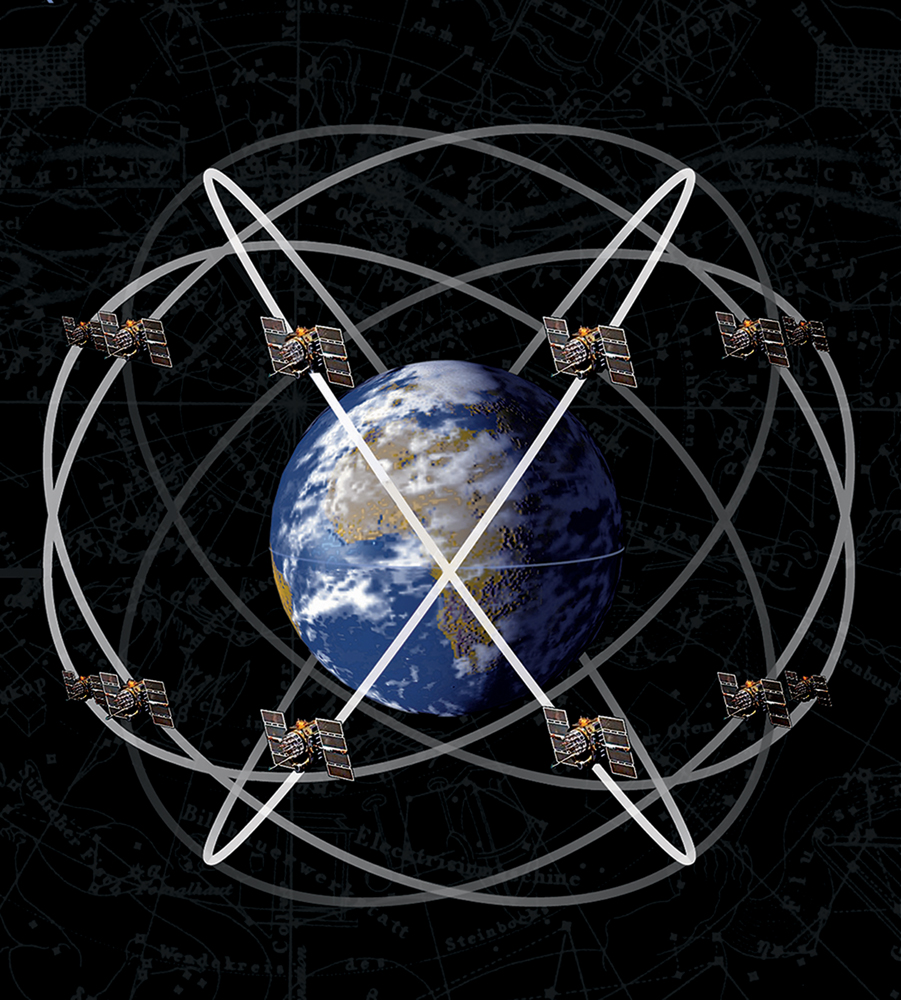
\includegraphics[width=\textwidth]{images/satelliten_schaubild.jpg}
            \end{figure}
            {\small [TimeAndNavigation]}
        \end{column}
    \end{columns}
\end{frame}

\begin{frame}{Die verschiedenen Satelliten im Überblick.}
    \begin{table}
        \begin{tabular}{c S[table-format=2.0] c S[table-format=2.1] c}
            \toprule
            {} & {Aktiv} & {Start} & {\enquote{MHD}} & {Änderungen} \\
            \midrule
            IIA   &  1 & 1990-1997 & 7.5 & \\
            IIR   & 11 & 1997-2004 & 7.5 & Onboard Uhrüberwachung \\
            IIR-M &  7 & 2005-2009 & 7.5 & Mehr und stärkere M(ilitär)signale \\
            IIF   & 12 & 2010-2016 & 12  & neue Uhr, bessere Signalabstrahlung \\
            III   &  0 & Dez 2018  & 15  & bessere Zuverlässigkeit, kein SA mehr \\
            IIIF  &  0 & Dez 2018  & 15  & $^{\---}"^{\---}$ , SAR kompatibel \\
            \bottomrule
        \end{tabular}
    \end{table}
\end{frame}

\begin{frame}{SA = selective Availability}
    ziviles GPS stören\\
    Grund: \textit{national security reasons}\\
    Abschaltung: 02.05.2000, 4 Uhr
    \begin{figure}
        \centering
        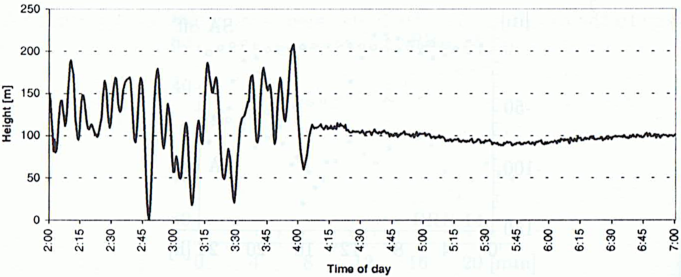
\includegraphics[width=\textwidth]{images/sa-hoehe.PDF}
    \end{figure}
    Höhenmessung in Kootwijk (Niederlande), 02.05.2000\;\;{\small [C,H-W,L](S.90)}
\end{frame}

\begin{frame}{GPS-Satelliten}
    \begin{columns}
        \begin{column}{0.5\textwidth}
            \begin{figure}
                \centering
                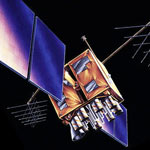
\includegraphics[height=0.6\textheight]{images/IIR.jpg}
            \end{figure}
            \centering{Typ IIR}
        \end{column}
        \begin{column}{0.5\textwidth}
            \begin{figure}
                \centering
                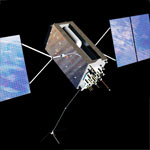
\includegraphics[height=0.6\textheight]{images/IIIA.jpg}
            \end{figure}
            \centering{Typ III}
        \end{column}
    \end{columns}~\\~\\
    Komponenten: Atomuhr, Solarpanele, Antennen, Computer \;\;{\small [gps.gov]}
\end{frame}

\begin{frame}{NIST-7 Atomuhr}
    \begin{figure}
        \centering
        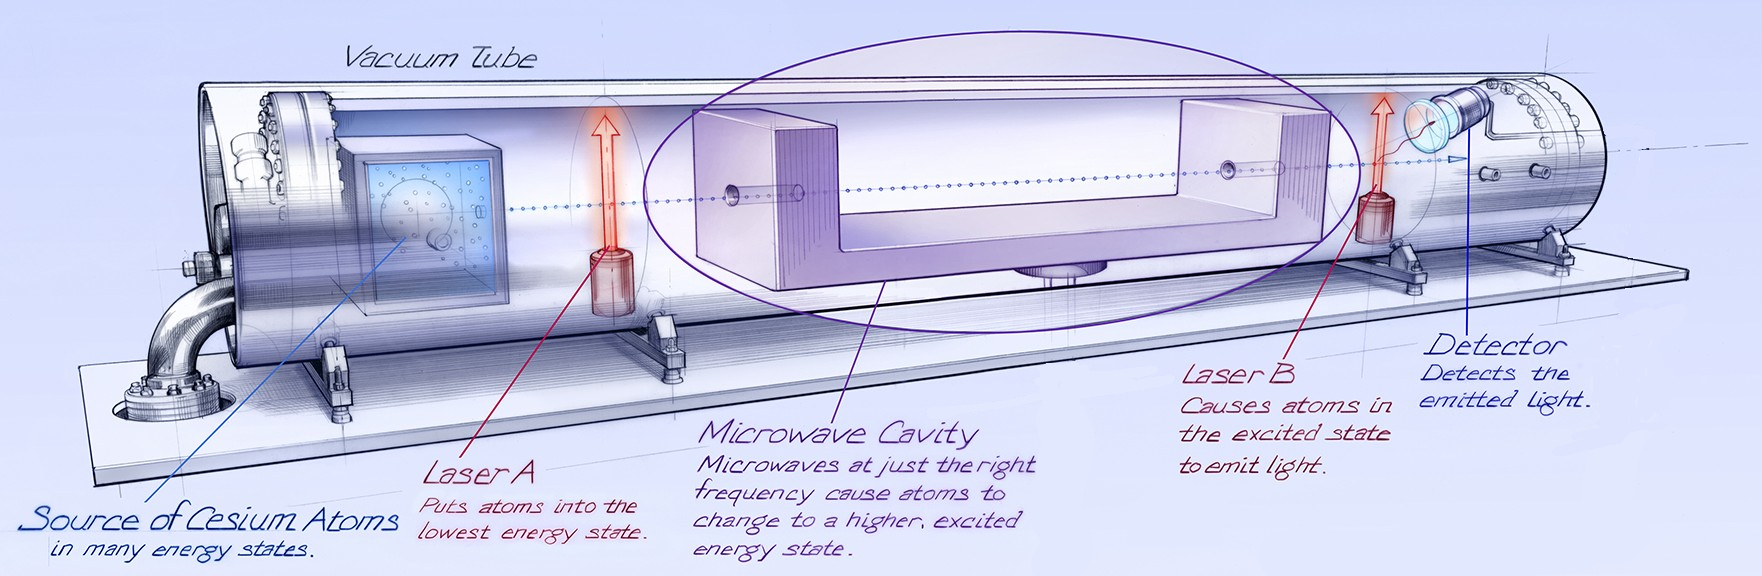
\includegraphics[width=\textwidth]{images/nist-7.jpg}
    \end{figure}
    \begin{columns}
        \begin{column}{0.5\textwidth}
            \begin{figure}
                \centering
                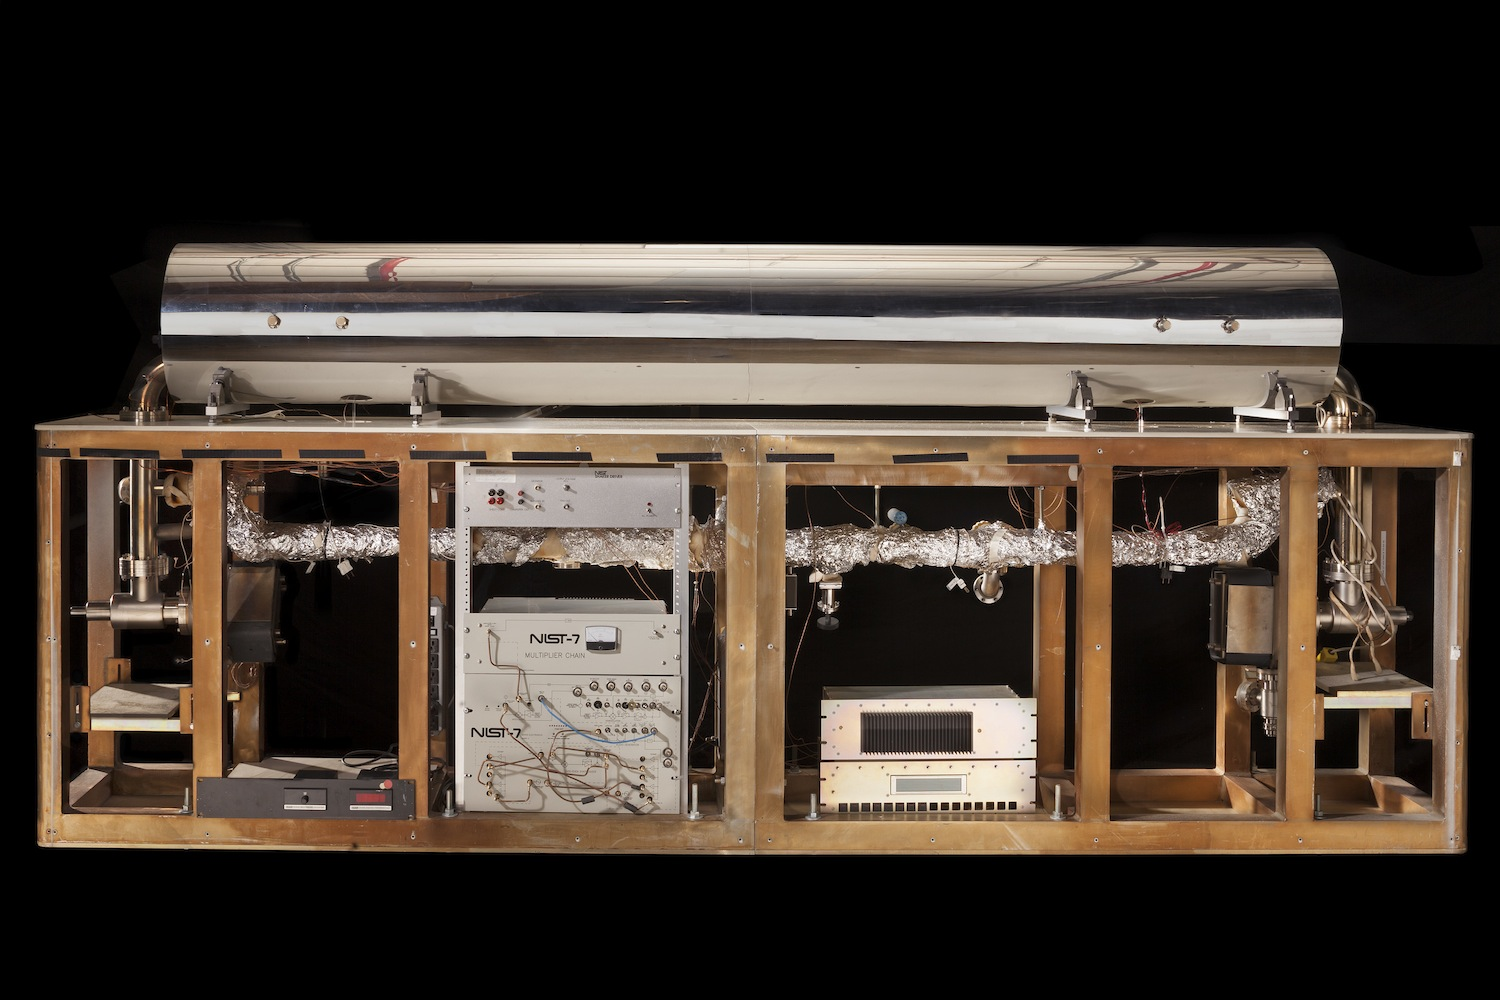
\includegraphics[height=0.4\textheight]{images/nist-7-real.jpg}
            \end{figure}
        \end{column}
        \begin{column}{0.5\textwidth}
            Ähnliche Methode zur Bestimmung\\
            von $\SI{1}{\second}$ als SI-Grundheiten\\
            {\small [TimeAndNavigation]}
        \end{column}
    \end{columns}
\end{frame}
